% Derived from the TeX Live PGF decorations.pathreplacing manual.
\documentclass[border=2pt]{standalone}
\usepackage{tikz}
\usetikzlibrary{decorations.pathreplacing}
\begin{document}
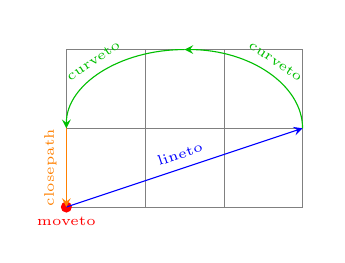
\begin{tikzpicture}[>=stealth, every node/.style={midway, sloped, font=\tiny},
  decoration={show path construction,
    moveto code={
      \fill [red] (\tikzinputsegmentfirst) circle (2pt)
        node [fill=none, below] {moveto};},
    lineto code={
      \draw [blue,->] (\tikzinputsegmentfirst) -- (\tikzinputsegmentlast)
        node [above] {lineto};
    },
    curveto code={
      \draw [green!75!black,->] (\tikzinputsegmentfirst) .. controls
        (\tikzinputsegmentsupporta) and (\tikzinputsegmentsupportb)
        ..(\tikzinputsegmentlast) node [above] {curveto};
    },
    closepath code={
      \draw [orange,->] (\tikzinputsegmentfirst) -- (\tikzinputsegmentlast)
        node [above] {closepath};}
  }]
  \draw [help lines] grid (3,2);
  \path [decorate] (0,0) -- (3,1) arc (0:180:1.5 and 1) -- cycle;
\end{tikzpicture}
\end{document}
